\documentclass[12pt]{extarticle}
\usepackage[english,ukrainian]{babel}
\usepackage[utf8]{inputenc}
\usepackage{amsmath,amssymb}
\usepackage{parskip}
\usepackage{graphicx}
\usepackage{xcolor}
\usepackage{tcolorbox}
\tcbuselibrary{skins}
\usepackage[framemethod=tikz]{mdframed}
\usepackage{chngcntr}
\usepackage{enumitem}
\usepackage{hyperref}
\usepackage{float}
\usepackage{subfig}
\usepackage{chngcntr}
\usepackage{esint}

\usepackage[top=2.5cm, left=3cm, right=3cm, bottom=4.0cm]{geometry}
\usepackage[table]{xcolor}

\usepackage{algorithm}
\usepackage{algpseudocode}
\usepackage{listings}
\usepackage{xcolor}

\definecolor{codegreen}{rgb}{0,0.6,0}
\definecolor{codegray}{rgb}{0.5,0.5,0.5}
\definecolor{codepurple}{rgb}{0.58,0,0.82}
\definecolor{backcolour}{rgb}{0.95,0.95,0.92}

\lstdefinestyle{mystyle}{
    backgroundcolor=\color{backcolour},   
    commentstyle=\color{codegreen},
    keywordstyle=\color{magenta},
    numberstyle=\tiny\color{codegray},
    stringstyle=\color{codepurple},
    basicstyle=\ttfamily\footnotesize,
    breakatwhitespace=false,         
    breaklines=true,                 
    captionpos=b,                    
    keepspaces=true,                 
    numbers=left,                    
    numbersep=5pt,                  
    showspaces=false,                
    showstringspaces=false,
    showtabs=false,                  
    tabsize=2
}
\lstset{style=mystyle}

\usepackage{ragged2e}
\begin{document}

\begin{titlepage}
	\centering
	
\includegraphics[width=0.15\textwidth]{images/lab_1/logo.png}\par\vspace{0.3cm}
	{\textbf{Міністерство освіти і науки України}\par
 Харківський національний університет імені В.Н. Каразіна\par}
    \vspace{1cm}
	{\Large \textsc{Лабораторна робота \#2}\par
    \textbf{Інтерполяція функцій сплайнами: кубічні інтерполяційні сплайни}\par}
	\vfill
 \begin{FlushRight}
	\textbf{Виконав:}\par Захаров Дмитро Олегович \par Група МП-31
\end{FlushRight}
	\vfill

% Bottom of the page
	{\large Харків -- 2023\par}
\end{titlepage}

\tableofcontents
\pagebreak

\section{Постановка задачі}

Побудувати інтерполяційні кубічні сплайни $S_n(x)$ для функції $f: [\alpha,\beta] \to \mathbb{R}$, заданої в узлах:
\begin{enumerate}
    \item $x_k = \alpha+k\cdot h, \; h = \frac{\beta-\alpha}{n}, \; k \in \{0,\dots,n\}$
    \item $\hat{x}_k = \frac{1}{2}\left(\beta+\alpha -(\beta-\alpha)\cos \frac{2k+1}{2(n+1)}\pi\right), \; k \in \{0,\dots,n\}$
\end{enumerate}

значеннями $\{f_i\}_{i=0}^n$. 

На друк вивести результати у вигляді таблиць:
\[
x_i^* \; \; \; \; \; f(x_i^*) \; \; \; \; \; S_n(x_i^*) \; \; \; \; \; |f(x_i^*) - S_n(x_i^*)|
\]
де $x_i^*=x_i+\alpha h, \; i \in \{0,\dots,n-1\}, \alpha \in (0,1)$.

\textbf{Варіант 5.} $\alpha=0,\beta=1$,
\[
f(x) = x^3 + \cos x + e^{\frac{x}{10}} \sin x
\]

\pagebreak
\section{Опис методу}

\subsection{Кубічний інтерполяційний сплайн}

\textit{Кубічним інтерполяційним сплайном} $S(x)$ для функції $f \in \mathcal{C}[\alpha,\beta]$ для вузлів $\{x_i\}_{i=0}^n \subset [\alpha,\beta]$ називається функція, що має наступні властивості:
\begin{enumerate}
    \item $S(x)$ є кубічним многочленом на відрізку між суміжними вузлами. Формально:
    \[
    S(x) = a_0^{[i]}x^3 + a_1^{[i]}x^2 + a_2^{[i]}x + a_3^{[i]}, \; x \in [x_{i-1},x], \; i \in \{1,\dots,n\}
    \]
    \item $S \in \mathcal{C}^2[\alpha,\beta]$
    \item $S(x_i) = f(x_i) \, \forall i \in \{0,\dots,n\}$
    \item $S''(\alpha)=S''(\beta)=0$ (кубічний сплайн дефекту 1)
\end{enumerate}

\subsection{Теорема про знаходження кубічного інтерполяційного сплайну}\label{sub:2-2}

\textbf{Теорема.} Умови, що зазначені вище, однозначно визначають кубічний інтерполяційний сплайн $S(x)$, дефекту 1, що має вигляд:
\begin{align*}
S(x) = \frac{m_{i-1}(x_i-x)^3}{6h_i} + \frac{m_i(x-x_{i-1})^3}{6h_i} \\ + \left(f(x_{i-1}) - \frac{h_i^2 m_{i-1}}{6}\right) \frac{x_i-x}{h_i} + \left(f(x_i)-\frac{h_i^2m_i}{6}\right) \frac{x - x_{i-1}}{h_i}
\end{align*}
для $x \in [x_{i-1},x], \; i \in \{1,\dots,n\}$ де числа $m_i$ є розв'язком системи рівнянь:
\[
\begin{cases}
    m_0 = 0 
    \\
    \frac{h_im_{i-1}}{6} + \frac{h_i+h_{i+1}}{3}m_i + \frac{h_{i+1}m_{i+1}}{6} = -\frac{f(x_i)-f(x_{i-1})}{h_i} + \frac{f(x_{i+1})-f(x_i)}{h_{i+1}},\; i \in \{1,\dots,n-1\} 
    \\
    m_n = 0
\end{cases}
\]
де ми позначили $h_i := x_i - x_{i-1}, \; i \in \{1,\dots,n\}$. 

\subsection{Метод прогонки}\label{sub:2-3}

Нехай маємо лінійне рівняння виду $\boldsymbol{A}\mathbf{x} = \mathbf{b}$ де матриця $\boldsymbol{A} \in \mathbb{R}^{n \times n}$ має вигляд:
\[
\boldsymbol{A} = \begin{bmatrix}
    d_1 & u_1 & 0 & 0 & \dots & 0 \\
    \ell_2 & d_2 & u_2 & 0 & \dots & 0 \\
    0 & \ell_3 & d_3 & u_3 & \dots & 0 \\
    \vdots & \vdots & \ddots & \ddots & \dots & \vdots \\
    0 & 0 & 0 & \dots & \ell_n & d_n
\end{bmatrix}
\]

Існує швидкий спосіб знаходження розв'язку $\mathbf{x}=[x_1,\dots,x_n]^{\top}$, який називають методом прогонки. Для цього спочатку знаходять наступні значення (прямий хід):
\[
\alpha_i = -\frac{u_i}{\ell_i\alpha_{i-1} + d_i}, \; \beta_i = \frac{b_i - \ell_i\beta_{i-1}}{\ell_i\alpha_{i-1} + d_i}, \; i \in \{1,\dots,n\}
\]
де для зручності ми поклали $\ell_1=u_n=0$. Далі застосовуємо зворотний хід:
\begin{align*}
x_n = \beta_n, \\
x_{i-1} = \alpha_{i-1}x_i + \beta_{i-1}, \; i \in \{n,n-1,\dots,2\}
\end{align*}
для знаходження $x_i$. 

\subsection*{Знаходження кубічного сплайну}

Поєднуючи ідеї розділів \ref{sub:2-2} та \ref{sub:2-3}, можемо знайти коефіцієнти $m_i$, що потрібні для побудови $S(x)$. З розділу \ref{sub:2-2} перепишемо рівняння для знаходження $m_i$ наступним чином:
\[
\begin{bmatrix}
    \frac{h_1+h_2}{3} & \frac{h_2}{6} & 0 & 0 & \dots & 0 & 0 
    \\
    \frac{h_2}{6} & \frac{h_2+h_3}{3} & \frac{h_3}{6} & 0 & \dots & 0 & 0 \\
    0 & \frac{h_3}{6} & \frac{h_3+h_4}{3} & \frac{h_4}{6} & \dots & 0 & 0 \\
    0 & 0 & \frac{h_4}{6} & \frac{h_4+h_5}{3} & \dots & 0 & 0 \\
    \vdots & \vdots & \vdots & \vdots & \ddots & \vdots & \vdots \\
    0 & 0 & 0 & 0 & \dots & \frac{h_{n-1}}{6} & \frac{h_{n-1}+h_n}{3}
\end{bmatrix}\begin{bmatrix}
    m_1 \\ m_2 \\ m_3 \\ \vdots \\ m_{n-2} \\ m_{n-1}
\end{bmatrix} = \begin{bmatrix}
    -\frac{f(x_1)-f(x_0)}{h_1} + \frac{f(x_2)-f(x_1)}{h_2} \\ 
    -\frac{f(x_2)-f(x_1)}{h_2} + \frac{f(x_3)-f(x_2)}{h_3} \\
    -\frac{f(x_3)-f(x_2)}{h_3} + \frac{f(x_4)-f(x_3)}{h_4} \\
    \vdots \\ 
    -\frac{f(x_{n-2})-f(x_{n-3})}{h_{n-2}} + \frac{f(x_{n-1})-f(x_{n-2})}{h_{n-1}} \\
    -\frac{f(x_{n-1})-f(x_{n-2})}{h_{n-1}} + \frac{f(x_{n})-f(x_{n-1})}{h_{n}}
\end{bmatrix}
\]

Тобто в нашому випадку $\ell_i = \frac{h_i}{6}, u_i = \frac{h_{i+1}}{6}, d_i = \frac{h_i+h_{i+1}}{3},b_i = -\frac{f(x_i)-f(x_{i-1})}{h_i} + \frac{f(x_{i+1})-f(x_i)}{h_{i+1}}$. Далі, застосовуючи метод прогонки з розділу \ref{sub:2-3}, легко знаходимо $m_i$.

\pagebreak
\section{Текст програми}

Повний текст програми можна знайти за \href{https://github.com/ZamDimon/University-Homeworks/tree/main/Term%205/Numerical%20Analysis/code/lab_2}{цим посиланням} ($\leftarrow$ напис клікабельний) на \textit{Github} сторінку.

\subsection{Генерація вузлів}

Для початку, створимо файл \texttt{generators.py}, завантажимо залежності та створимо свій тип для інтервалу:

\begin{lstlisting}[language=Python, caption=Завантаження залежностей]
from math import cos, pi
from typing import Tuple, TypeAlias, List
from abc import ABC, abstractmethod

Interval: TypeAlias = Tuple[float, float]
\end{lstlisting}

Зробимо генерацію вузлів через абстрактний клас, котрий буде вміти створюватись та генерувати набір $x$ координат вузлів через функцію \texttt{generate\_nodes}. Також, тут же задамо функцію \texttt{generate\_test\_points}, котра буде видавати набір $x$ координат точок, на котрих ми будемо оцінювати інтерполяцію (як сказано в умові, використовуючи формулу $x_i^* = x_i+\alpha h$ де $x_i$ це координата вузла).

\begin{lstlisting}[language=Python, caption=Задання абстрактного класу]
class IDataPointsGenerator(ABC):
    """Interface for generating data points"""
    
    def __init__(self, interval: Interval, number: int) -> None:
        """
        Function initializing the generator

        ### Args:
        - interval (`Interval`): Interval on which the data points will be generated
        - number (`int`): Number of data points to generate
        """
        
        assert number > 0, "Number of data points must be greater than 0"
        assert interval[0] < interval[1], "Lower bound must be less than upper bound"
        
        self._lower, self._upper = interval
        self._number = number
    
    @abstractmethod
    def generate_nodes(self) -> List[float]:
        """
        Function generating data points

        ### Returns:
            `List[float]`: List of generated x coordinates
        """
        pass
    
    @abstractmethod
    def generate_test_points(self, alpha: float = 0.1) -> List[float]:
        """
        Function generating test points for evaluating the polynomial
        ### Args:
        - alpha (`float`): We will evaluate the polynomial at points x_i + alpha*h

        Returns:
        - List[float]: List of x coordinates
        """
        
        nodes = self.generate_nodes()
        h = (self._upper - self._lower) / self._number
        return [node + alpha*h for node in nodes]
\end{lstlisting}

Далі, наводимо конкретні реалізації цього інтерфейсу.

\subsubsection{Лінійно розбитий проміжок}
\begin{lstlisting}[language=Python, caption=Генерація лінійно розкинутих точок]
class LinearDataPointsGenerator(IDataPointsGenerator):
    """Class for generating linearly spaced data points"""
    
    def __init__(self, interval: Interval, number: int) -> None:
        super().__init__(interval, number)
    
    def generate_nodes(self) -> List[float]:
        fn = lambda i: self._lower + i * (self._upper - self._lower) / (self._number)
        return [fn(i) for i in range(self._number + 1)]
    
    def generate_test_points(self, alpha: float = 0.1) -> List[float]:
        return super().generate_test_points(alpha)
\end{lstlisting}

\subsubsection{Проміжок розбитий по гармонічному закону}
\begin{lstlisting}[language=Python, caption=Генерація точок по закону з косинусом]
class CosineDataPointsGenerator(IDataPointsGenerator):
    """Class for generating cosine spaced data points"""
    
    def __init__(self, interval: Interval, number: int) -> None:
        super().__init__(interval, number)
        
    def generate_nodes(self) -> List[float]:
        fn = lambda i: 0.5*(self._lower+self._upper-(self._upper-self._lower)*cos((2*i+1)*pi/(2*(self._number+1))))
        return [fn(i) for i in range(self._number + 1)]

    def generate_test_points(self, alpha: float = 0.1) -> List[float]:
        return super().generate_test_points(alpha)
\end{lstlisting}

\subsubsection{Перевірка генерації}
Перевіримо роботу програми, поклавши $n:=4$ для нашого конкретного інтервалу $[-2,2]$. В коді, це виглядає так:

\begin{lstlisting}[language=Python, caption=Використання генераторів]
linear_generator = LinearDataPointsGenerator((-2.0, 2.0), 4)
cosine_generator = CosineDataPointsGenerator((-2.0, 2.0), 4)

print(f"Linear generator nodes: {linear_generator.generate_nodes()}")
print(f"Cosine generator nodes: {cosine_generator.generate_nodes()}")
\end{lstlisting}

Якщо запустити, отримаємо наступний результат:

\begin{lstlisting}[language=bash, caption=Результат запуску генераторів]
Linear generator nodes: [-2.0, -1.0, 0.0, 1.0, 2.0]
Cosine generator nodes: [-1.902113032590307, -1.1755705045849463, -1.2246467991473532e-16, 1.175570504584946, 1.902113032590307]
\end{lstlisting}

Перевіримо аналітично. У випадку лінійного розбиття, маємо:
\[
x_k = -2 + k \cdot \frac{2+2}{4} = -2 + k
\]

Дійсно, якщо підставляти $k \in \{0,\dots,4\}$, отримаємо точки $\{-2,-1,0,1,2\}$.

У випадку розбиття по косинусу:
\[
\hat{x}_k = \frac{1}{2}\left(2-2-(2+2)\cos \frac{2k+1}{10}\pi\right) = -2 \cos \frac{(2k+1)\pi}{10}
\]

Тому, наприклад, $\hat{x}_0 = -2\cos \frac{\pi}{10} \approx -1.902$. Аналогічно можна перевірити схожість для інших $k$. Отже, ми дійсно отримали схожі результати.

\subsection{Метод прогонки}

Створимо файл \texttt{solver.py} та реалізуємо алгоритм \ref{sub:2-3} у функції \texttt{tridiagonal\_matrix\_algorithm} котра приймає набір нижньодіагональних елементів $\{\ell_i\}_{i=2}^n$, наддіагональних елементів $\{u_i\}_{i=1}^{n-1}$, діагональні елементи $\{d_i\}_{i=1}^n$ та праву частину системи $\{b_i\}_{i=1}^n$ і повертає розв'язок рівняння:

\begin{lstlisting}[language=Python, caption=Реалізація методу прогонки]
import numpy as np

def tridiagonal_matrix_algorithm(
    l: np.ndarray, 
    u: np.ndarray, 
    d: np.ndarray, 
    b: np.ndarray
) -> np.ndarray:
    """
    Solve a system of linear equations with the tridiagonal matrix algorithm.
    ### Args:
        l (List[float]): Lower diagonal
        u (List[float]): Upper diagonal
        d (List[float]): Main diagonal
        b (List[float]): Right hand side
    ### Returns:
        List[float]: Solution to the system of linear equations
    """
    assert len(l) == len(u) == len(d) - 1 == len(b) - 1, "Invalid input shapes"
    
    l = np.insert(l, 0, 0.0, axis=0) # Add zero to the beginning of the list
    u = np.append(u, 0.0) # Add zero to the end of the list
    n = len(d) # Number of equations
     
    # Forward substitution
    alpha, beta = np.zeros(n), np.zeros(n)
    for i in range(n):
        alpha[i] = -u[i] / (l[i] * alpha[i-1] + d[i])
        beta[i] = (b[i] - l[i] * beta[i-1]) / (l[i] * alpha[i-1] + d[i])
      
    # Backward substitution
    x = np.zeros(n) # Defining a solution
    x[n-1] = beta[n-1]
    for i in range(n-2, -1, -1):
        x[i] = alpha[i] * x[i+1] + beta[i]
    return x
\end{lstlisting}

\subsection{Кубічний сплайн}

Створимо файл \texttt{spline.py} та завантажимо залежності:

\begin{lstlisting}[language=Python, caption=Завантаження залежностей]
from math import prod
import numpy as np
import solver

from abc import ABC, abstractmethod
from typing import List, Tuple, TypeAlias

Point: TypeAlias = Tuple[float, float]
\end{lstlisting}

Зокрема, ми завантажили \texttt{solver.py} з попереднього розділу.

Задамо абстракцію для інтерполяційної функції (буде корисно, якщо у майбутньому це доведеться робити знову):

\begin{lstlisting}[language=Python, caption=Інтерфейс для інтерполяційної функції]
class IInterpolate(ABC):
    """Interface any interpolating function should implement"""
    
    def __init__(self, points: List[Point]) -> None:
        """ 
        Initializes the interpolating function
        ### Args:
        - points (`List[Point]`): List of points to interpolate on
        """
        assert len(points) > 1, "At least two points are required"
        self._points = points
    
    @abstractmethod
    def evaluate(self, x: float) -> float:
        """
        Evaluates the interpolating function at x
        ### Args:
        - x (`float`): Point to evaluate the polynomial at
        ### Returns:
            `float`: Value of the polynomial at x
        """
        pass
\end{lstlisting}

Далі, наводимо реалізацію кубічного сплайну

\begin{lstlisting}[language=Python, caption=Реалізація кубічного сплайну]
class CubicSpline(IInterpolate):
    """Cubic spline interpolating function"""
    
    def __init__(self, points: List[Point]) -> None:
        super().__init__(points)
        
        # Defining the number of points
        self._n = len(points)
        # Finding h_{i} = x_{i} - x_{i-1}
        self._differences = self._find_differences()
        # Finding m_{i} coefficients
        self._m = self._find_m_coefficients()
        
    def _find_differences(self) -> np.ndarray:
        """ Generates a list of pairwise differences between x coordinates of points

        Returns:
            np.ndarray: numpy array of length n-1 where n is the number of points
        """
        return np.array([self._points[i][0] - self._points[i-1][0] for i in range(1, self._n)])
        
    def _find_m_coefficients(self) -> np.ndarray:
        """ Generates a list of m coefficients needed for the evaluation

        Returns:
            np.ndarray: numpy array of length n where n is the number of points
        """
        l = np.array([self._differences[i] / 6.0 for i in range(1, self._n-2)]) # Initializing the lower diagonal
        u = np.array([self._differences[i+1] / 6.0 for i in range(self._n-3)]) # Initializing the upper diagonal
        d = np.array([(self._differences[i] + self._differences[i+1]) / 3.0 for i in range(self._n-2)]) # Initializing the main diagonal
        b = np.array([-(self._points[i][1] - self._points[i-1][1]) / self._differences[i-1]
             + (self._points[i+1][1] - self._points[i][1]) / self._differences[i] for i in range(1, self._n-1)]) # Initializing the right hand side

        m = solver.tridiagonal_matrix_algorithm(l, u, d, b)
        m = np.insert(m, 0, 0.0, axis=0) # Add zero to the beginning of the list
        m = np.append(m, 0.0) # Add zero to the end of the list
        return m
     
    def evaluate(self, x: float) -> float:
        # Defining a list of terms to sum
        for i in range(1, self._n):
            if self._points[i-1][0] <= x <= self._points[i][0]:
                return self._m[i-1] * (self._points[i][0] - x)**3 / (6.0 * self._differences[i-1]) \
                    + self._m[i] * (x - self._points[i-1][0])**3 / (6.0 * self._differences[i-1]) \
                    + (self._points[i-1][1] - self._m[i-1] * self._differences[i-1]**2 / 6.0) * (self._points[i][0] - x) / self._differences[i-1] \
                    + (self._points[i][1] - self._m[i] * self._differences[i-1]**2 / 6.0) * (x - self._points[i-1][0]) / self._differences[i-1]
                    
        raise ValueError("x is not in the interval")
\end{lstlisting}

Пару коментарів по реалізації:
\begin{enumerate}
    \item Ми знаходимо елементи $\{m_i\}_{i=0}^n$ за допомогою функції \texttt{\_find\_m\_coefficients} під час ініціалізації.
    \item У функції \texttt{evaluate} ми проходимось по всім парам точок і коли знаходимо потрібній сегмент, підставляємо все у формулу з розділу \ref{sub:2-2}.
\end{enumerate}

\subsection{Програма для оцінки}

Тепер напишемо програму, котра оцінює сплайн і видає потрібні нам таблиці. Створюємо файл \texttt{cli.py} і знову завантажуємо залежності:
\begin{lstlisting}[language=Python, caption=Завантаження залежностей]
# Math imports
from math import exp, sin, cos
import numpy as np

# Internal imports
from generators import Interval, IDataPointsGenerator, LinearDataPointsGenerator, CosineDataPointsGenerator
from spline import CubicSpline

# Rich logging
from rich.console import Console
from rich.table import Table

import matplotlib.pyplot as plt
from typing import Callable
\end{lstlisting}


Далі створюємо функцію, що створює 2 генератора, наш сплайн і будує 2 таблиці, як і просили у умові:

\begin{lstlisting}[language=Python, caption=Реалізація побудови таблиць з результатами]
def evaluate_accuracy(
    fn: Callable[[float], float],
    interval: Interval,
    segments_number: int = 20,
    alpha: float = 0.2,
) -> None:
    """Evaluates the accuracy of the spline

    ### Args:
    - fn (Callable[[float], float]): Function to interpolate
    - interval (`Interval`): Interval on which to plot the polynomial
    - segments_number (int, optional): _description_. Defaults to 20.
    - alpha (float, optional): Alpha parameter for the test points. Defaults to 0.2.
    """
    
    # Defining the generator and defining a set of points
    generators: dict[str, IDataPointsGenerator] = {
        "linear generation": LinearDataPointsGenerator(interval, segments_number),
        "cosine generation": CosineDataPointsGenerator(interval, segments_number)
    }
    
    # For rich logging
    console = Console()
    
    for generator_name, generator in generators.items():
        # Defining the points on which to interpolate the polynomial
        node_x = generator.generate_nodes()
        node_points = [(x, fn(x)) for x in node_x]
        
        # Defining the spline
        spline = CubicSpline(node_points)
        
        # Defining the test points
        test_x = generator.generate_test_points(alpha=alpha)
        test_points = [(x, fn(x)) for x in test_x]
        
        table = Table(title=f"Spline evaluation using {generator_name}")
        table.add_column("x", justify="center", style="cyan", no_wrap=True)
        table.add_column("f(x)", justify="center", style="magenta")
        table.add_column("S(x)", justify="center", style="green")
        table.add_column("|f(x)-S(x)|", justify="center", style="blue")
    
        for test_point in test_points[:-1]:
            x_label = "{:.18f}".format(test_point[0])
            f_x_label = "{:.18f}".format(test_point[1])
            p_x_label = "{:.18f}".format(spline.evaluate(test_point[0]))
            difference_label = "{:.18f}".format(abs(test_point[1] - spline.evaluate(test_point[0])))
            
            table.add_row(x_label, f_x_label, p_x_label, difference_label)

        console.print(table)
\end{lstlisting}

Також додатково побудуємо 2 графіки для порівняння: один буде зображати функцію $f(x)$ на проміжку $[\alpha,\beta]$, а другий сплайн $S(x)$:
\begin{lstlisting}[language=Python, caption=Побудова графіків]
def plot_polynomial(
    fn: Callable[[float], float],
    interval: Interval,
    segments_number: int = 2,
) -> None:
    """
    Plots the polynomial and the spline on the same plot
    
    ### Args:
    - fn (`Callable[[float], float]`): Function to plot
    - interval (`Interval`): Interval on which to plot the polynomial
    - segments_number (`int`): Number of segments to use for the spline
    
    ### Returns:
    Displayed polynomial and spline
    """
    
    # Defining the spline
    generator = LinearDataPointsGenerator(interval, segments_number)
    node_x = generator.generate_nodes()
    node_points = [(x, fn(x)) for x in node_x]
    spline = CubicSpline(node_points)
    
    x = np.arange(*interval, 0.02)
    plt.figure()
    plt.subplot(211)
    plt.plot(x, [fn(x) for x in x], 'b', x, [spline.evaluate(x) for x in x], 'r--')
    plt.show()
\end{lstlisting}

Нарешті, викликаємо ці дві функції послідовно, ініціалізувавши нашу функцію і проміжок:
\begin{lstlisting}[language=Python, caption=Вхід на програму]
if __name__ == "__main__":
    # Defining the task parameters
    interval = (0.0, 1.0)
    segments_number = 20
    alpha = 0.2
    fn = lambda x: x**3 + cos(x) + exp(x / 10.0) * sin(x)
    
    # Evaluating the accuracy
    evaluate_accuracy(fn, interval, segments_number=segments_number, alpha=alpha)
    
    # Plotting the polynomial
    plot_polynomial(fn, interval, segments_number=3)
\end{lstlisting}

Для побудови графіків ми скористалися $3$ сегментами, оскільки для більшої кількості функції повністю накладаються.

\pagebreak

\section{Результати}

Для експериментів ми взяли $n=20$ та $\alpha=0.2$. Якщо ви хочете спробувати вибрати інші параметри, то можете запустити програму, що прикріплена у додатку :)

\subsection{Лінійно розбитий проміжок}
\begin{figure}[H]
    \centering
    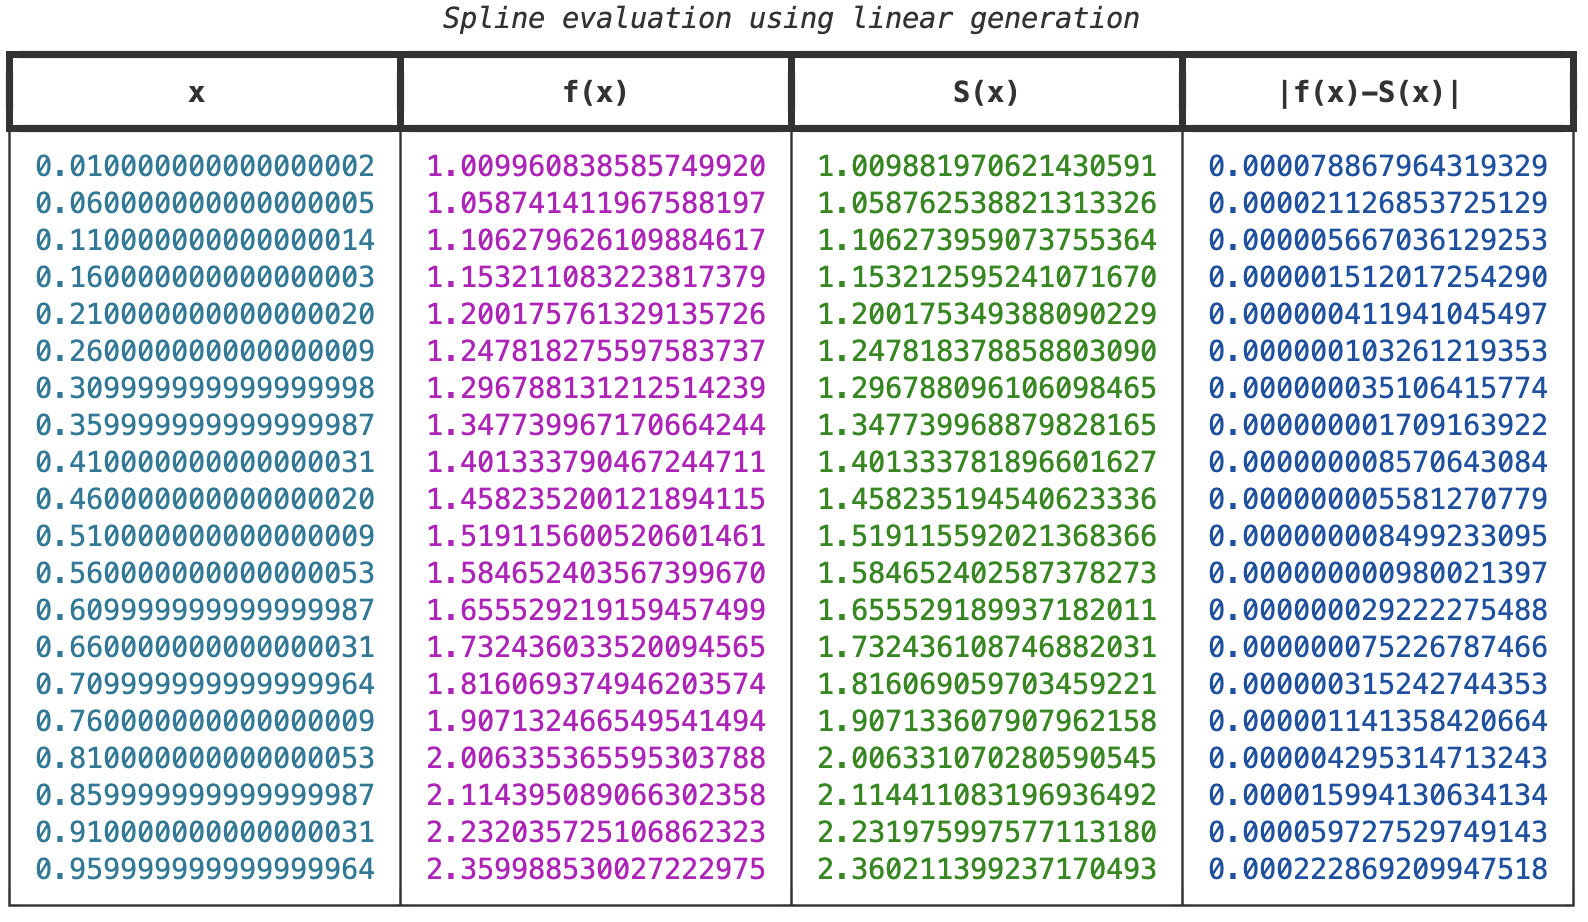
\includegraphics[width=\textwidth]{images/lab_2/spline_linear.png}
    \caption{Результат для сплайну для лінійного розбиття}
    \label{fig:1}
\end{figure}

Графік, на якому ми зобразили порівняння сплайну та функції:
\begin{figure}[H]
    \centering
    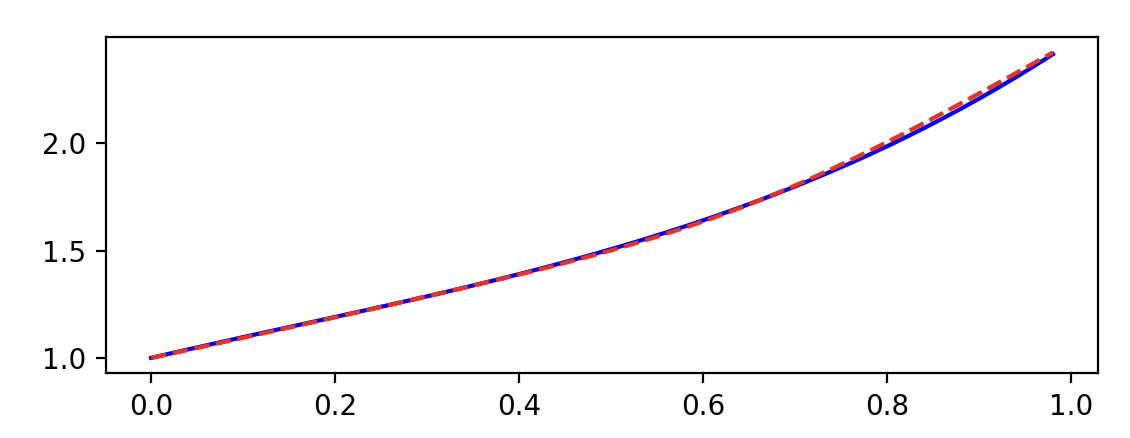
\includegraphics[width=\textwidth]{images/lab_2/plot.png}
    \caption{Порівняння сплайну та функції. \textcolor{blue}{синім} ми намалювали графік, а \textcolor{red}{червоним} пунктиром -- сплайн}
    \label{fig:2}
\end{figure}

\subsection{Проміжок розбитий по гармонічному закону}

\begin{figure}[H]
    \centering
    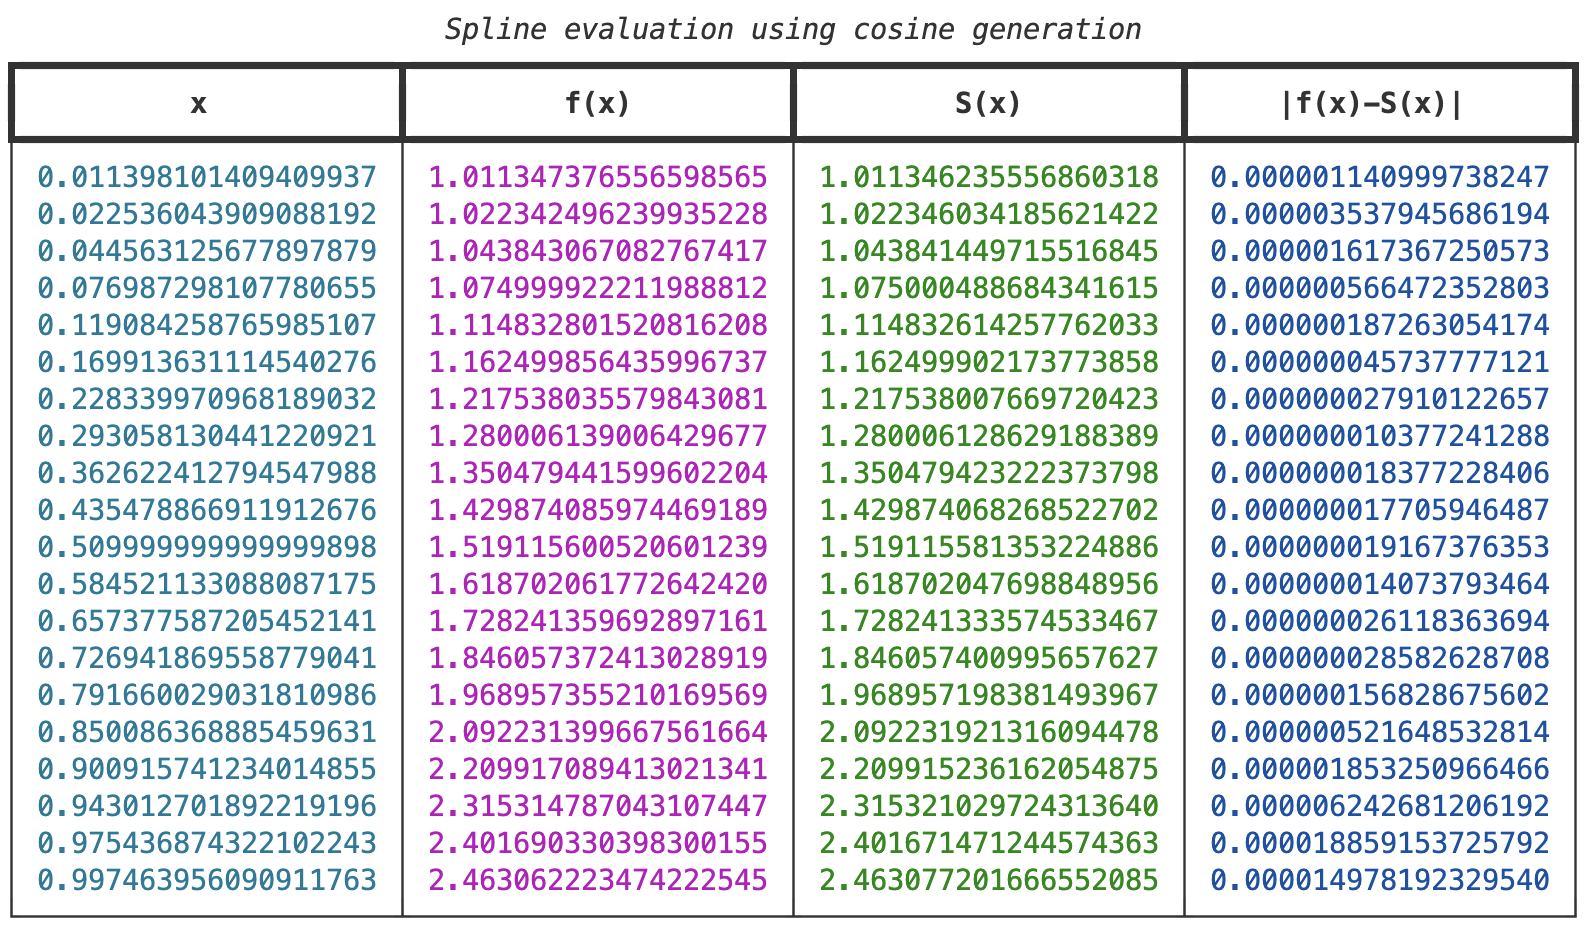
\includegraphics[width=\textwidth]{images/lab_2/spline_cosine.png}
    \caption{Результат для сплайну для розбиття по косинусу}
    \label{fig:3}
\end{figure}
\vspace{5px}

\pagebreak
\section{Висновки}

В цій лабораторній роботі ми:
\begin{itemize}
\item навчилися будувати кубічний сплайн теоретично;
\item навчилися писати комп'ютерну програму (на прикладі мови \texttt{Python}), що будує кубічний сплайн;
\item оцінювати написану програму та діставати дані з експериментів.
\end{itemize}

Також, як бачимо, модуль різниці $|f(x^*)-S(x^*)|$ -- дуже мала величина, що говорить про точність інтерполяції на заданому проміжку (оскільки ми брали набір точок $x^*_i$, що відносно близький до вузлів $x_i$).

\end{document}

